\documentclass[a4paper, openany]{memoir}

\usepackage[utf8]{inputenc}
\usepackage[T1]{fontenc} 
\usepackage[english]{babel}

\usepackage{fancyhdr}
\usepackage{fancyvrb}
\usepackage{float}
\usepackage{amsmath, amsthm, amssymb}
\usepackage{enumitem}
\usepackage[bookmarksopen=true,bookmarksopenlevel=2]{hyperref}
\usepackage{indentfirst}
\usepackage[normalem]{ulem}
\usepackage{graphicx}

\usepackage{listings}
\usepackage{xcolor}

\pagestyle{fancy}
\fancyhf{}
\fancyhead[LE]{\leftmark}
\fancyhead[RO]{\rightmark}
\fancyhead[RE, LO]{Database Systems}
\fancyfoot[LE, RO]{\thepage}
\fancyfoot[RE, LO]{Pete Gautam}

\renewcommand{\headrulewidth}{1.5pt}

\definecolor{codegreen}{rgb}{0,0.6,0}
\definecolor{codegray}{rgb}{0.5,0.5,0.5}
\definecolor{codepurple}{rgb}{0.58,0,0.82}
\definecolor{backcolour}{rgb}{0.95,0.95,0.92}

\lstdefinestyle{thestyle}{
    backgroundcolor=\color{backcolour},
    basicstyle=\ttfamily\footnotesize,
    keywordstyle=\color{red!80}\bfseries,
    ndkeywordstyle=\color{blue!80}\bfseries,
    identifierstyle=\color{black},
    commentstyle=\color{codegreen},
    stringstyle=\color{codepurple},
    breakatwhitespace=false,
    breaklines=true,
    captionpos=b,
    keepspaces=true,
    % numberstyle=\tiny\color{codegray},
    % numbers=left,
    % numbersep=2pt,
    showspaces=false,
    showstringspaces=false,
    showtabs=false,          
    tabsize=2
}

\lstset{style=thestyle}

\chapterstyle{thatcher}

\begin{document}
\chapter{Relational Design}
\section{Database Fundamentals}
Human activity is data-driven. We are making decisions, proceeding with actions and reasoning, based on observed data. However, we are limited in storing all data in memory and recalling them. So, we define a robust base that can store, update and delete and search data efficiently. This is a database.

\subsection{Data Management System}
The fundamental functionality of a data management system is to:
\begin{itemize}
    \item provide a data model, e.g. relational data model, object-oriented data model, etc.
    \item provide access to data, i.e. query, insert, delete and update
    \item provide tools to analyse data, i.e. complex aggregation queries (e.g. count the number of queries that satisfy a condition), histograms, etc.
    \item store data physically, from memory to hard disks.
    \item store data securely, by using control access to sensitive and confidential data and by encoding data.
    \item maintain data consistency, e.g. in the face of failures (e.g. software bugs, power cuts), and recover from failures.
    \item optimise data access to efficiently retrieve data, using indexing and hashing data structures along with optimisation algorithms.
\end{itemize}

In terms of the user, the database system is a black box with an interface for users/applications offering the functionalities we discussed. We allow the user to write commands in high-level language that can be translated into machine code. To do this, we make use of a declarative programming language (e.g. SQL). This allows us to manage and query data. It is declarative since we tell the database what to do, and not how to do it, e.g. we say find a tuple that matches the query, not what kind of searching algorithm to use in order to find the tuple.

In terms of systems engineering, the database system is a set of interconnected components, as shown below.
\begin{figure}[H]
    \centering
    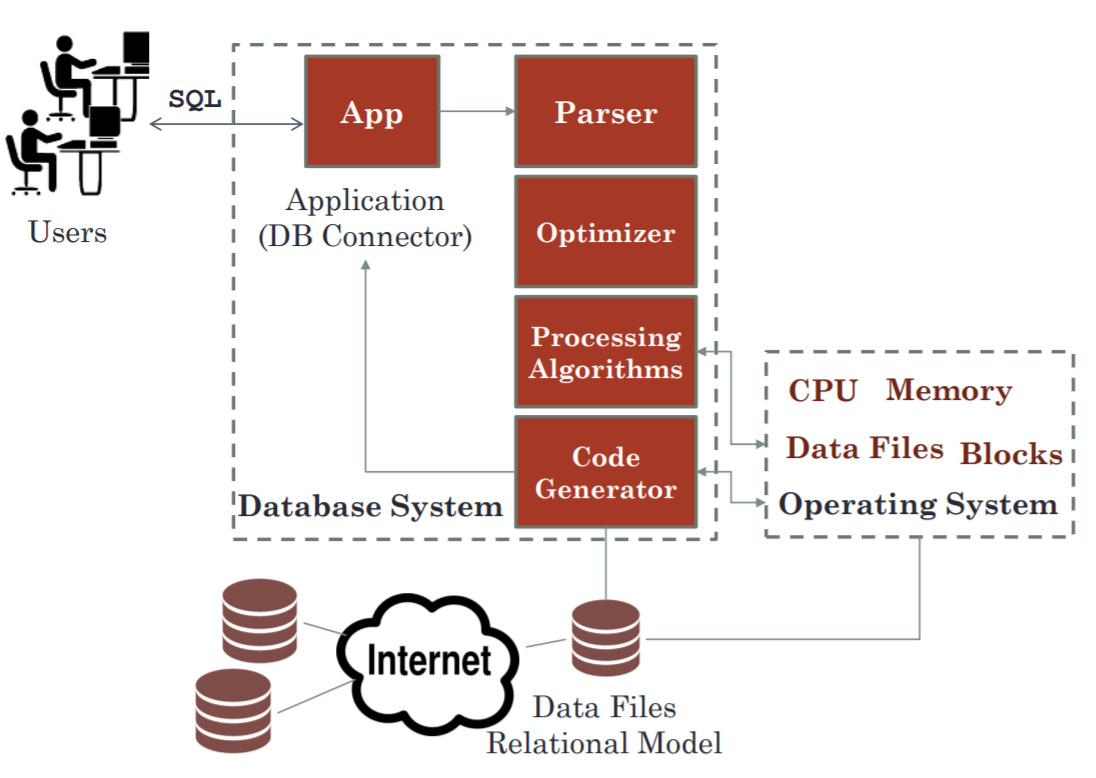
\includegraphics[scale=0.4]{src/Database Systems SE.PNG}
\end{figure}
\noindent When a user queries the database using SQL, we parse and optimise the query, and then processes the algorithm (which talks to the CPU, memory, data files). Then, the operating system generates the code that we can run to the data files in order to retrieve the relevant tuples. We might require the internet to access the data files.

\subsection{Data}
There are 3 families of data:
\begin{itemize}
    \item structured data- well-defined data structure, e.g. tables where we understand what the data represents;
    \item unstructured data- less information is provided on interpreting such data, e.g. web pages, texts, sensor measurements.
    \item semi-structured data- self-descriptive data, e.g. XML or JSON.
\end{itemize}
Modern data management systems can manage all families of data.

\newpage

\section{Relational Model}
We will transform a textual description of a real problem into a set of concepts conveying exactly the same information. There are 2 ways of doing this: Entity-relationship (ER) modelling, and Relational modelling. 

ER modelling does not guarantee optimality in operations and query executions. On the other hand, relational modelling is mathematics-driven. It uses relational algebra, set theory and functional dependency theory. This guarantees query optimisation based on the 4 fundamental operations (search, update, add, delete).

A conceptual data model is a mathematical model for interpreting our data. The interpretation involves the following concepts:
\begin{itemize}
    \item the entities, e.g. students, employees;
    \item the attributes, e.g. name, address;
    \item the relationships, e.g. an employee works in a department, a student attends many courses.
\end{itemize}

In the relational conceptual model, we allow any entity to relate to other entities given that they share a common attribute(s) (i.e. the foreign key). For example, we can model books being borrowed in the library with 2 entities- readers and books. A reader has attributes: name, age, book title and id. A book has attributes: book title, subject, ISBN, number of pages. We can create a relation between books and readers using the common attribute book title.

Any entity and relationship are both called relations. It can be thought of as a 2-dimensional table. A column in this table is an ordered collection of attributes, while a row in this table is a tuple that represents an instance of the relation. Moreover, there has to be an attribute that uniquely identifies each tuple.

By representing data as tables, we can easily perform operations on it. In particular, we can list attributes of interest to be retrieved, and/or constrained attributes to filter out irrelevant tuples. For example, a query can to be return the names of the customers with active accounts and balance greater than £500. So, the attribute of interest is name, and the constrains are: active accounts and balance greater than £500. We can represent this in SQL as well.
\begin{lstlisting}[language=SQL]
SELECT Name 
FROM BankAccount 
WHERE Balance > 500 AND Status = "active"
\end{lstlisting}
Clearly, the language is declarative- we merely specify what to find, not how to find it.

Now, we will formalise the relational model. The schema of a relation is $R(A_1, A_2, \dots, A_n)$. Here, $R$ is the name of the relation, and the values $A_1, A_2, \dots, A_n$ are a tuple of attributes. Each attribute $A_i$ assumes values in a domain $D_i$. For example, a schema is: 
\begin{verbatim}
BankAccount(AccountNumber, Name, Balance, Status),
\end{verbatim}
where:
\begin{itemize}
    \item the value of \texttt{accountNumber} is a natural number;
    \item the \texttt{name} is a character with length at most 50;
    \item the value of the \texttt{balance} is a real number; and
    \item the \texttt{status} is either \texttt{active} or \texttt{inactive}- it is an enumerated type.
\end{itemize}

A tuple of a relation $R$ is an order set of values corresponding to the attributes of $R$ satisfying the domain constrains (i.e. the value of tuple at index $i$ lives in the domain $D_i$). It is denoted $t = (v_1, v_2, \dots, v_n)$, with $v_i \in D_i$. We can also directly access the value of the attribute $v_i$ by $t[v_i]$. An instance $r(R)$ is a set of tuples.

The relational model also allows the value of an entity to be \texttt{null}. We use this value to represent a value that is either unknown, inapplicable, uncertain, or missing. So, the relational database scheme is a set of relations $S = \{R_1, R_2, \dots, R_n\} \cup \{\texttt{NULL}\}$.

\subsection{Relational constraints}
Relational constraints are conditions that must hold on all instances for each relation. There are 3 fundamental constraints:
\begin{itemize}
    \item Key constraint- a key uniquely identifies a tuple in a relation;
    \item Entity integrity constraint- keys cannot be null;
    \item Referential integrity constraint- for two relations to have a relationship, they must share attribute(s).
\end{itemize}

A superkey (SK) of a relation $R$ is a set of attributes that contains at least one attribute that uniquely identifies a tuple. That is, for $t_1, t_2 \in r(R)$,
\[t_1 \neq t_2 \implies t_1[SK] \neq t_2[SK].\]
For example, consider the following relation
\begin{verbatim}
Employee (SSN, EName, LName, BDate, Salary, DNO).
\end{verbatim}
Then, the subsets:
\begin{itemize}
    \item $\{\texttt{SSN}, \texttt{EName}, \texttt{BDate}\}$ contains \texttt{SSN}, which is unique for each attribute- it is a superkey;
    \item $\{\texttt{SSN}\}$, is also a superkey;
    \item $\{\texttt{EName}, \texttt{Salary}\}$ might not identify a tuple uniquely- it is not a superkey.
\end{itemize}

A candidate key is the minimal superkey, i.e. the set with the smallest number of attributes that can uniquely identify tuples. Formally, the set $K = \{A_1, A_2, \dots, A_k\}$ is a candidate key if $K$ is superkey and for all $j \in \{1, 2, \dots, k\}$, $K \setminus \{A_j\}$ is not a superkey. That is, removing any attribute from $K$ will mean that it is no longer a superkey. 

In the example above, $\{\texttt{SSN}, \texttt{EName}, \texttt{BDate}\}$ is not a candidate key since $\{\texttt{SSN}, \texttt{BDate}\}$ is still a superkey. In fact, the only candidate key is $\{\texttt{SSN}\}$. If a relation has several candidate keys, then we can arbitrarily chosen one of them to be a primary key (PK). The others are called secondary keys. This is the key constraint. We underline the PK in the relation schema.

In an instance $r(R)$, the value of the PK within any tuple cannot be \texttt{NULL}. If the PK is composed of many attributes, we do not allow any of the attributes to be \texttt{NULL}. This is the entity integrity constraint. 

For a relationship from the referencing relation $R_1$ to the referenced relation $R_2$, there has to exist an attribute (or a set of attributes), called the Foreign Key (FK), in $R_1$ that either has the same value with the PK in $R_2$ or is \texttt{NULL}. That is,
\[t_1[FK] \text{ references } t_2[PK] \implies t_2[PK] = t_1[FK] \text{ or } t_1[FK] = \texttt{NULL}.\]
So, the value of the foreign key, if not null, must be an existing primary key. Note that this is one-directional. It is still possible for us to have a primary key whose value is never a foreign key. This is denoted by a directed arc from $R1.FK$ to $R2.PK$.

\newpage

\section{Functional Dependency}
Functional Dependency Theory is used to quantify the degree of goodness of a relational schema. Goodness is in terms of the attributes, e.g. PK and FK. To quantify the degree of goodness, we introduce the normal forms. We also need to judge whether there are pitfalls to the relational model. The relational schema should also be efficient in terms of the insertion, deletion and update operations. We should convey as much information as possible while minimising redundancy (repetition of data and uncertainities). 

\subsection{Informal guidelines for relational schema}
There are 4 informal guidelines used to judge a relational schema, that we will consider below.

The first guideline is that the attributes of a relation should make sense. So, attributes of different entities, e.g. students and courses should not be stored within the same relation completely. Our objective is to minimise redundancy between relations, so we should store different entities separately.

Any relationship between relations should only be represented through Foreign Keys and Primary Keys, e.g. if we have a student taking a set of courses, we should have 3 relations- one for students, one for courses, and one for their relationship 
\begin{Verbatim}[commandchars=+\[\]]
STUDENT_COURSE(+underline[GUID], +underline[COURSE_ID], TUTORIAL_GROUP),
\end{Verbatim}
where \texttt{GUID} and \texttt{COURSE\_ID} are primary keys of the relations student and course respectively.

The second guideline is that we should avoid redundant tuples. Having repeated tuples means:
\begin{itemize}
    \item the storage cost increases, since we need to store redundant tuples.
    \item the inconsistency cost and operation anomalies also increases, because we the replicas need to be kept consistent during insertion, deletion and update of tuples.
    \item the replicas might result in consistency anomalies.
\end{itemize}
When we delete a tuple, we need to delete other tuples that depend on this tuple- we cascade the deletion operation. When we update a tuple, we need to update other tuples similarly- we propagate the update operation. We must do this to maintain consistency within the schema.

Assume that we have a relation schema containing only the following relation:
\begin{Verbatim}[commandchars=+\[\]]
EMP_PROJ(+underline[SSN], +underline[PNumber], Hours, EName, PName, PLocation).
\end{Verbatim}
This relation stores the number of hours an employee is working on a project per week. Within an instance of this relation, we expect there to be a repetition of many attributes within many tuples, e.g. if an employee is working on many projects. 

Now, assume that we have 600 employees working on the project \texttt{PNumber = 2} with \texttt{PName = ProductY}. We want to change the name of the project \texttt{ProductY} to \texttt{ProductZ}. To enforce consistency, we need to change all the 600 tuples. This is very inefficient for such a small change. If we didn't do this update, then some employees would be working on an inexistent project. Ideally, we should only have to update one tuple.

Next, if we wanted to delete the project with \texttt{PNumber = 2}, then we would need to delete all the tuples with \texttt{PNumber = 2}. However, we might be removing some employees from the relation by doing so. In the business logic, it might be the case that they get assigned to a default project- we should not have to delete the tuples.

The third guideline is that relations should have as few \texttt{NULL} values as possible. We might have \texttt{NULL} values if:
\begin{itemize}
    \item the value is not applicable or invalid;
    \item a value is not known; or
    \item a value is not available.
\end{itemize}
Attributes that are frequently \texttt{NULL} should be placed in separate relations to avoid wasting storage and reducing uncertainty.

For example, consider the following relation: 
\begin{Verbatim}[commandchars=+\[\]]
EMPLOYEE(+underline[SSN], Name, Phone1, Phone2, Phone3)
\end{Verbatim}
In a particular instance of the relation, we might find that only 10 of the 1600 employees have three contact numbers. So, we have 1590 null values in that column, which wastes a lot of storage. We should create another relation for the third contact number: \texttt{PHONE3(\underline{SSN}, Phone3)}, along with the original relation \texttt{EMPLOYEE(\underline{SSN}, Name, Phone1, Phone2)}. Then, we only need to store 10 tuples in the Phone3 relation, which saves a lot of storage.

The fourth guideline is that we should design relations to avoid fictitious tuples after join. A fictitious tuple is one that was not present in the original relation. We illustrate this with an example. So, consider the relation
\begin{Verbatim}[commandchars=+\[\]]
EMP_PROJ(+underline[SSN], +underline[PNumber], Hours, EName, PName, PLocation)
\end{Verbatim}
As we saw before, this is a bad relation with respect to delete and update anomalies. So, we can break it into 2 relations: 
\begin{Verbatim}[commandchars=+\[\]]
R1(+underline[SSN], Ename, +underline[PNumber], PName, PLocation)
R2(Hours, +underline[PLocation])
\end{Verbatim}
The shared attribute for the 2 relations is \texttt{PLocation}. 
To retrieve information from the two relations, we need to join them with respect to \texttt{PLocation}. In particular, assume that we want to find the working hours per week for each employee. To do this, we would need to join \texttt{R1} and \texttt{R2} on the common attribute \texttt{PLocation}. This is an issue, since it creates tuples which did not exist in \texttt{EMP\_PROJ}.

We illustrate this with an example. So, we have 3 relations:
\begin{Verbatim}[commandchars=+\[\]]
R(SSN, PName, PLocation, Hours)
Q(SSN, PName, Hours)
P(PLocation, Hours)
\end{Verbatim}
Assume that we have 3 instances of \texttt{R}, given below:
\begin{table}[H]
    \centering
    \begin{tabular}{|c|c|c|c|}
        \hline
        \texttt{SSN} & \texttt{PName} & \texttt{PLocation} & \texttt{Hours} \\
        \hline
        111 & PR1 & Glasgow & 20 \\
        222 & PR1 & Glasgow & 10 \\
        333 & PR2 & Edinburgh & 23 \\
        \hline
    \end{tabular}
\end{table}
\noindent Then, we will have 3 instances of \texttt{Q} and \texttt{P}, given by
\begin{table}[H]
    \centering
    \begin{tabular}{|c|c|c|}
        \hline
        \texttt{SSN} & \texttt{PName} & \texttt{PLocation} \\
        \hline
        111 & PR1 & Glasgow \\
        222 & PR1 & Glasgow \\
        333 & PR2 & Edinburgh \\
        \hline
    \end{tabular}
\end{table}
\begin{table}[H]
    \centering
    \begin{tabular}{|c|c|}
        \hline
        \texttt{PLocation} & \texttt{Hours} \\
        \hline
        Glasgow & 20 \\
        Glasgow & 10 \\
        Edinburgh & 23 \\
        \hline
    \end{tabular}
\end{table}
\noindent So, when we join the two tables \texttt{Q} and \texttt{P} with respect to the attribute \texttt{PLocation} we get the following table:
\begin{table}[H]
    \centering
    \begin{tabular}{|c|c|c|c|}
        \hline
        \texttt{SSN} & \texttt{PName} & \texttt{PLocation} & \texttt{Hours} \\
        \hline
        \textbf{111} & \textbf{PR1} & \textbf{Glasgow} & \textbf{10} \\
        111 & PR1 & Glasgow & 20 \\
        222 & PR1 & Glasgow & 10 \\
        \textbf{222} & \textbf{PR1} & \textbf{Glasgow} & \textbf{20} \\
        333 & PR2 & Edinburgh & 23 \\
        \hline
    \end{tabular}
\end{table}
\noindent We have ended up with 2 fictitious tuples here, which are highlighted in bold. So, we need to choose the right common attribute in order to avoid fictitious tuples.

\subsection{Formal guidelines for relational schema}
Functional Dependency (FD) is a formal metric to measure the goodness of a relational schema. In particular, FD is a constraint derived from the relationship between attributes. 

Given a relation, we say that the attribute $X$ functionally determines the attribute $Y$ if a value of $X$ determines a unique value for $Y$. So, the value of $Y$ can be reconstructed given the value of $X$. We denote $X \to Y$ to mean that $X$ (uniquely) determines $Y$. Mathematically, we say that if two tuples have the same value for attribute $X$, then they have the same value for attribute $Y$. That is, for tuples $t_1, t_2$,
\[t_1[X] = t_2[X] \implies t_1[Y] = t_2[Y].\]
This is a constraint on all the instances of $R$.

We illustrate this with an example. Consider the relation
\[\texttt{EMP\_PROJ(\underline{SSN}, \underline{PNumber}, Hours, EName, PName, PLocation)}.\]
The following is an instance of the relation.
\begin{table}[H]
    \centering
    \begin{tabular}{|c|c|c|c|c|c|}
        \hline
        \texttt{SSN} & \texttt{PNumber} & \texttt{Hours} & \texttt{EName} & \texttt{PName} & \texttt{PLocation} \\
        \hline
        1 & 5 & 10 & Chris & PX & G12 \\
        2 & 5 & 30 & Stella & PX & G12 \\
        1 & 7 & 15 & Chris & PY & G45 \\
        \hline
    \end{tabular}
\end{table}
\noindent Here, \texttt{SSN} determines \texttt{EName}. In the first and the third tuple, the \texttt{SSN} values match and so the \texttt{ENmae} values also match. So, we have a FD \texttt{SSN} $\to$ \texttt{EName}. That is, social security number determines the name of an employee, which makes sense.

Moreover, \texttt{PNumber} determines \texttt{PName}. In the first and the second tuple, the \texttt{PNumber} values match and so the \texttt{PName} values also match. So, we have FD \texttt{PNumber} $\to$ \texttt{PName}.

There is also another FD. Since $\{\texttt{SSN}, \texttt{PNumber}\}$ is a primary key, these two attributes have to determine all the other attributes. So, $\{\texttt{SSN}, \texttt{PNumber}\} \to \{\texttt{Hours}, \texttt{EName}, \texttt{PName}, \texttt{Location}\}$.

We will now look at some properties of FDs:
\begin{itemize}
    \item If $K$ is a candidate key, then $K$ functionally determines all attributes in $R$, i.e. $K \to R$. The converse is also true.
    
    \item If $Y \subseteq X$, then $X \to Y$, e.g. if $X = \{\texttt{SSN}, \texttt{EName}\}$, then
    \[X \to \{\texttt{SSN}\}, \qquad X \to \{\texttt{EName}\}, \qquad X \to X.\]
    This is called reflexivity.
    
    \item If $X \to Y$, then $X \cup Z \to Y \cup Z$. This is called augmentation.
    
    \item If $X \to Y$ and $Y \to Z$, then $X \to Z$. This is called transitivity.
\end{itemize}

\newpage

\section{Normalisation Theory}
The theory of normalisation is the progressive decomposition of unsatisfactory (bad) relations by breaking up their attributes into smaller, better relations. We will exploit the FDs to specify which attributes can be PKs and FKs. This is the normalisation theory. We do this by:
\begin{itemize}
    \item asserting which are the FDs among the attributes using the given specification;
    \item creating a (big) relation with all the attributes;
    \item recursively decompose the relation based on FDs into many smaller subrelations such that when we re-join them, it guarantees that no information is lost and reconstructs the big relation without any fictitious tuples.
\end{itemize}

There are different degrees of decomposition, referred to as Normal Form (NF):
\begin{itemize}
    \item First normal form (1NF),
    \item Second normal form (2NF),
    \item Third normal form (3NF), and
    \item Boyce-Codd normal form (BCNF).
\end{itemize}
The higher the normal form, the better optimised the schema is.

A prime attribute is an attribute that belongs to some candidate key of the relation, and a non-prime attribute is not a prime attribute, i.e. it is not a member of any candidate key. For example, in the relation
\begin{Verbatim}[commandchars=+\[\]]
EMP_PROJ(+underline[SSN], +underline[PNumber], Hours, EName, PName, PLocation)
\end{Verbatim}
the attributes \texttt{SSN} and \texttt{PNumber} are prime attributes, while \texttt{Hours}, \texttt{EName}, \texttt{PName}, \texttt{PLocation} are non-prime attributes.

\subsection{1NF}
In the first normal form, the domain $D_i$ of each attribute $A_i$ in a relation $R$ refers only to atomic (simple, indivisible) values. So, 1NF disallows nested and multi-valued attributes. We expect there to be redundant and repeated values.

\subsection{2NF}
In 2NF, we will break the record into multiple records to reduce redundancy. For this, we define full and partial FD. A full FD $X \to Y$ means that if we remove a prime attribute $A$ from the primary key $X$, then $X \setminus \{A\}$ does not functionally determine $Y$ anymore. That is,
\[X \setminus \{A\} \not\to Y.\]
Otherwise, we say that the FD $X \to Y$ is partial. For example, in the relation 
\begin{Verbatim}[commandchars=+\[\]]
EMP_PROJ(+underline[SSN], +underline[PNumber], Hours, EName, PName, PLocation),
\end{Verbatim}
$\{\texttt{SSN}, \texttt{PNumber}\} \to \texttt{Hours}$ is a full FD. This is because neither $\texttt{SSN} \to \texttt{Hours}$ or $\texttt{PNumber} \to \texttt{Hours}$ is true. But, $\{\texttt{SSN}, \texttt{PNumber}\} \to \texttt{EName}$ is a partial FD since $\texttt{SSN} \to \texttt{EName}$ is true.

We say that a relation $R$ is in 2NF if it is in 1NF and every non-prime attribute $A$ in $R$ is fully functionally dependent on the primary key of $R$. So, to transform a relation from 1NF to 2NF, we remove all the prime attributes from the primary key that cause partial dependencies. To do this, 
\begin{itemize}
    \item we identify all the partial FDs in the original relation (that is in 1NF);
    \item for each partial FD, we create a new relation such that all non-prime attributes in there are fully functionally dependent on the new primary key, i.e. the prime attribute in the original relation causing partial FDs.
\end{itemize}
Then, the new relation(s) will be in 2NF.

\subsection{3NF}
Consider the record below.
\begin{table}[H]
    \centering
    \begin{tabular}{|c|c|c|c|c|c|c|}
        \hline
        \texttt{\underline{SSN}} & \texttt{EName} & \texttt{BYear} & \texttt{Address} & \texttt{DNumber} & \texttt{DName} & \texttt{DMgr\_SSN} \\
        \hline
        1 & Chris & 1970 & A1 & 3 & SoCS & 12 \\
        2 & Stella & 1988 & A2 & 3 & SoCS & 12 \\
        3 & Philip & 2001 & A3 & 3 & SoCS & 12 \\
        4 & John & 1966 & A4 & 3 & SoCS & 12 \\
        5 & Chris & 1955 & A5 & 3 & SoCS & 12 \\
        6 & Anna & 1999 & A6 & 4 & Maths & 44 \\
        7 & Thalia & 2006 & A7 & 4 & Maths & 44 \\
        \hline
    \end{tabular}
\end{table}
\noindent This record is in 1NF- no entry contains more than one value. Moreover, the relation is in 2NF- since there is only one prime attribute, it must fully determine all the non-prime attributes. But the relation is still redundant. The last 3 attributes is the same in the first 5 and the last 2 rows. We could break this into 2 relations to avoid this redundancy. This will transform the record into 2 records, both of which are in 3NF.

If $X \to Z$ and $Z \to Y$, then $X \to Y$ by the transitivity property of FD. In particular, if $X$ is a prime attribute and $Z$ and $Y$ are non-prime attributes, then we say that $Y$ is transitively dependent on $X$ via $Z$. For example, In the record
\[\{\texttt{\underline{CourseID}, Lecturer, School}\},\]
we have FD1: \texttt{CourseID} $\to$ \texttt{Lecturer} and FD2: \texttt{Lecturer} $\to$ \texttt{School}. Moreover, we have FD3: \texttt{CourseID} $\to$ \texttt{School} via \texttt{Lecturer}, which is a non-prime attribute.

We say that a record $R$ is in 3NF if it is in 2NF and if there is no non-prime attribute which is transitively dependent on the primary key. So, all non-prime attributes are directly dependent on the PK.

\subsection{Generalised 3NF}
In 3NF, if $X \to Z$ and $Z \to Y$ and $X$ is a primary key, we only consider this to be a problem if $Z$ is a non-prime attribute. However, this still allows for some redundancy. For example, consider the following relation
\begin{Verbatim}[commandchars=+\[\]]
EMPLOYEE(+underline[SSN], PassportNo, Salary).
\end{Verbatim}
Then, we have the following FDs:
\begin{itemize}
    \item \texttt{SSN} $\to$ \texttt{PassportNo};
    \item \texttt{PassportNo} $\to$ \texttt{Salary};
    \item \texttt{SSN} $\to$ \texttt{Salary}.
\end{itemize}
The final FD is not a transitive FD since \texttt{PassportNo} is a prime attribute.

This gives rise to the generalised 3NF. Here, a non-prime attribute $A$ in relation $R$ is fully functionally dependent on every candidate key in $R$, and is non-transitively dependent on every candidate key in $R$. We still need to deal with prime attributes.

\subsection{BCNF}
Boyce-Codd Normal Form (BCNF) removes all inherent dependencies. Any attribute should be functionally dependent only on the PK. That is, a relation is in BCNF if whenever $X \to A$, then $X$ is the PK.

For example, consider the relation
\begin{Verbatim}[commandchars=+\[\]]
TEACH(+underline[Student], +underline[Course], Instructor)
\end{Verbatim}
with FDs: $\{\texttt{Student}, \texttt{Course}\} \to \texttt{Instructor}$ and $\texttt{Instructor} \to \texttt{Course}$. This relation satisfies 3NF since we cannot find a transitive FD from a prime attribute to a non-prime attribute. This is because there is only one non-prime attribute. Still, the relation is not in BCNF since \texttt{Instructor} $\to$ \texttt{Course} does not satisfy the BCNF condition. 

We need to decompose this record into 2 records. We need to ensure that we do not create fictitious tuples with this decomposition. The BCNF theorem tells us how to do this. If $R$ is a relation not in BCNF with $X \to A$ a FD that violates BCNF, then we can decompose $R$ to the following relations:
\begin{itemize}
    \item $R_1$ with attributes: $R \setminus A$, and
    \item $R_2$ with attributes: $X \cup A$.
\end{itemize}
If either $R_1$ or $R_2$ is still not in BCNF, we repeat the process.

\end{document}
